\documentclass[border=4pt]{standalone}
\usepackage{tikz}
\usetikzlibrary{arrows.meta}
\begin{document}
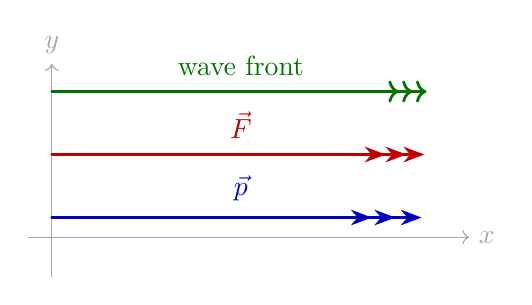
\begin{tikzpicture}[line cap=round]
  \draw[->,gray!70] (-.3,0) -- (5.3,0) node[right] {$x$};
  \draw[->,gray!70] (0,-.5) -- (0,2.2) node[above] {$y$};

  \draw[blue!75!black,line width=1pt,-{Stealth[sep=1pt] Stealth[sep=2pt] Stealth[sep=3pt]}]
    (0,.25) -- (4.8,.25) node[midway,above=2pt] {$\vec p$};
  \draw[red!75!black,line width=1pt,-{Stealth[sep=0pt] Stealth[sep=-1pt] Stealth[sep=2pt]}]
    (0,1.05) -- (4.8,1.05) node[midway,above=2pt] {$\vec F$};
  \draw[green!45!black,line width=1pt,-{[sep]>>>}]
    (0,1.85) -- (4.8,1.85) node[midway,above=2pt] {wave front};
\end{tikzpicture}
\end{document}
